\documentclass[11pt,a4paper]{article}
\usepackage[margin=2.2cm]{geometry}
\usepackage[T1]{fontenc}
\usepackage{lmodern}
\usepackage{graphicx}
\usepackage{booktabs}
\usepackage{amsmath}
\usepackage{amssymb}
\usepackage{xcolor}
\usepackage{caption}
\usepackage{subcaption}
\usepackage{float}
\usepackage{etoolbox}
\AtBeginEnvironment{table}{\small}
\usepackage{enumitem}
\usepackage[colorlinks=true,linkcolor=blue!50!black,urlcolor=blue!50!black,citecolor=blue!50!black]{hyperref}
\setlist{itemsep=2pt,topsep=4pt}
\emergencystretch=3em
\graphicspath{{../../results/}}
\newcommand{\code}[1]{\texttt{\detokenize{#1}}}

\title{$\Lambda \to p\pi^-$ in the ePIC B0 tracker --- update:\\hit seeding, the 5\,keV threshold, and $\Lambda$s up to 275\,GeV}
\author{Gadi Ninio}
\date{12 November 2026}

\begin{document}
\sloppy
\maketitle

\begin{abstract}
This note updates the report of 3 November 2026 (\code{docs/report/report.pdf}, ``the first
report''), which used truth-seeded B0 tracks from EICrecon main \code{8b44cae} and $\Lambda$s of
50--100\,GeV. Three things changed since. (1) The realistic B0 seeding of
\href{https://github.com/eic/EICrecon/pull/3116}{EICrecon\#3116} (triplets of B0 hits, no truth)
was built and compared with truth seeding on the same events: it finds a seed for every accepted
daughter, reconstructs every accepted proton, and gives 1--2 percentage points more fully
reconstructed $\Lambda$s (13.1\,\% instead of 12.0\,\% of the generated $\Lambda$s in the new
geometry) with the same mass peak. Its price is more tracks from secondaries, which matters only in
the thick old geometry. (2) The 5\,keV B0 threshold recommended in the first report is now the
EICrecon default (EICrecon\#3084). (3) New samples at 100--275\,GeV show that although the
probability that a $\Lambda$ decays before the B0 falls from 48\,\% to 17\,\% (p$\pi^-$, per
generated $\Lambda$), the early decays are reconstructed much better because the $\pi^-$ is harder,
so the fraction of fully reconstructed $\Lambda$s stays roughly flat up to 275\,GeV. One result is
not understood: the truth-seeded efficiency in the old geometry is much higher with the \#3116 build
than with main \code{8b44cae}.
\end{abstract}

\tableofcontents
\newpage

%=====================================================================================
\section{What changed since the first report}

\begin{table}[H]
\centering
\caption{Changes w.r.t.\ the first report.}
\begin{tabular}{@{}p{3.2cm}p{6cm}p{6.6cm}@{}}
\toprule
& first report (3 Nov) & this update (12 Nov)\\
\midrule
EICrecon & main \code{8b44cae} (local build) & EICrecon\#3116 branch at \code{1ca147b} = main of 2026-11-11 + \#3116 (contains \#2901 and \#3084)\\
B0 seeding & truth only (\#2901) & truth \emph{and} hit seeding, both written by the same job\\
B0 threshold & default 10\,keV; 5\,keV by option & 5\,keV is the default (\#3084, merged 2026-11-03)\\
eic-shell image & nightly of 2026-11-02 & nightly of 2026-11-07 (its \code{epic-main} already has the new B0)\\
old geometry & epic \code{43f427e} = geometry of the container & epic \code{43f427e}, built locally (\code{epic_43f427e}); same commit\\
new geometry & epic \code{ec774d8} (local build) & unchanged (= epic tag 26.11.0)\\
$\Lambda$ momentum & 50--100\,GeV & 50--100\,GeV (same simulated events, re-reconstructed) \emph{and} 100--275\,GeV (new)\\
\bottomrule
\end{tabular}
\end{table}

The definitions of the first report are unchanged (accepted daughter: its own simulated B0 hits
cover $\ge 3$ layers; tracking efficiency = reconstructed / accepted daughters; acceptance $\times$
efficiency per $p\pi^-$ decay). Two are added: the hit-seeded ``reconstructed daughter''
(Sec.~\ref{sec:hit}) and, as a cleaner denominator, ``per generated $\Lambda$''
(Sec.~\ref{sec:fates}). All macros take a \code{seeding} argument (\code{"truth"}, default, or
\code{"hit"}); \code{scripts/make_results.sh 07 08} produces every number of this note.

%=====================================================================================
\section{Hit seeding (EICrecon\#3116)}
\label{sec:hit}

\subsection{Status and method}
Realistic B0 seeding is not yet in EICrecon main. The first proposal, EICrecon\#3028, was closed on
2026-11-05 in favour of \#3116 (open); EICrecon\#3029, which shows as merged, is a bot include fix
merged into the branch of \#3028, not into main. \#3116 seeds B0 tracks with the ACTS triplet
seeder: one hit in each of three different B0 stations, the hits rotated so that the B0 dipole
field at the middle hit lies along $z$ (the ACTS seeder assumes a solenoid-like field), minimum
momentum across the field 1\,GeV, and tracks with $\ge 3$ measurements. There is no assumption on
the vertex or the charge, so it works for displaced decays by construction.

The chain is \code{B0TrackerSeeds} $\to$ \code{B0TrackerCKFTracks} (and\\
\code{B0TrackerCKFTrack[Unfiltered]Associations}) $\to$ \code{CombinedTracks} $\to$
\code{ReconstructedChargedParticles} (+\code{Associations}). The truth-seeded chain of \#2901 runs
in parallel in the same job (\code{ReconstructedTruthSeededChargedParticles}), so the two are
compared on identical events and hits. Hit seeds carry no MC link; a seed is assigned to a daughter
if at least two of its three hits were made by it (via \code{B0TrackerRawHitAssociations}).

The 1000-event samples of the first report (50--100\,GeV, seeds 101 and 102) were
re-reconstructed with the \#3116 build (\code{scripts/production/lambda_rereco.sh}); the
simulation is the same.

\subsection{Tracking efficiency}
\begin{table}[H]
\centering
\caption{Accepted daughters passing each step, proton / $\pi^-$, \#3116 build, 5\,keV, 1000 $\Lambda$ per geometry.}
\label{tab:steps}
\begin{tabular}{@{}lcccc@{}}
\toprule
step & old, truth & old, hit & new, truth & new, hit\\
\midrule
accepted & 404 / 349 & 404 / 349 & 295 / 240 & 295 / 240\\
rec.\ hits in $\ge 3$ layers & 100 / 100\,\% & 100 / 100\,\% & 100 / 100\,\% & 100 / 100\,\%\\
seed & 99 / 99\,\% & \textbf{100 / 100\,\%} & 97 / 96\,\% & \textbf{100 / 100\,\%}\\
CKF track & 98 / 66\,\% & 100 / 74\,\% & 94 / 61\,\% & 100 / 67\,\%\\
filtered track & 98 / 66\,\% & 100 / 73\,\% & 94 / 61\,\% & 100 / 65\,\%\\
\textbf{reconstructed particle} & \textbf{97.5 / 66.5\,\%} & \textbf{99.5 / 72.5\,\%} & \textbf{93.2 / 60.8\,\%} & \textbf{100 / 64.6\,\%}\\
\bottomrule
\end{tabular}
\end{table}

\begin{figure}[H]
\centering
\begin{subfigure}{0.49\textwidth}\centering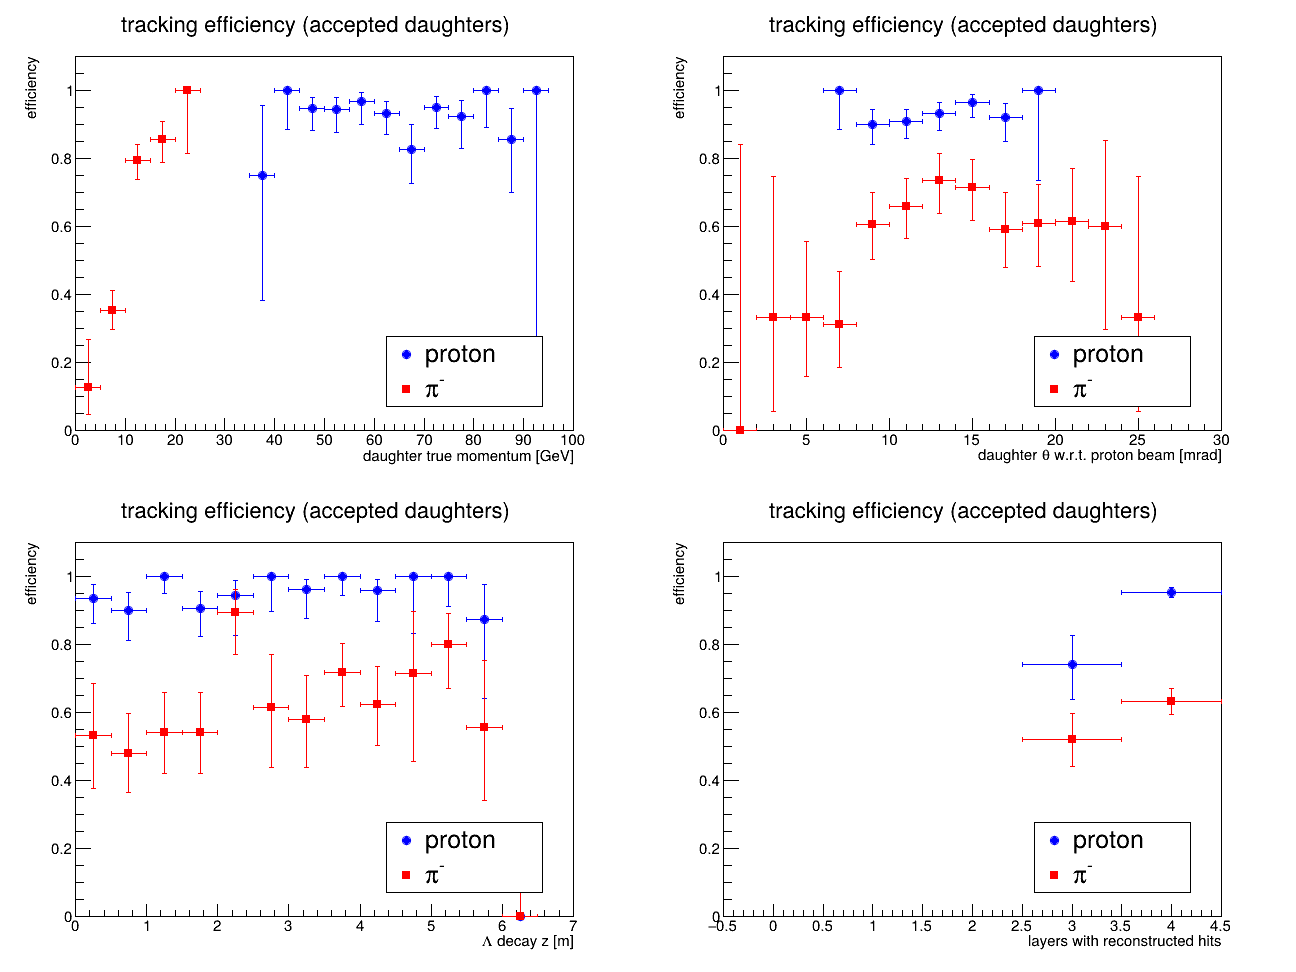
\includegraphics[width=\textwidth]{07_hit_seeding/tracking_efficiency_new_truth.png}\caption{new geometry, truth seeding}\end{subfigure}
\begin{subfigure}{0.49\textwidth}\centering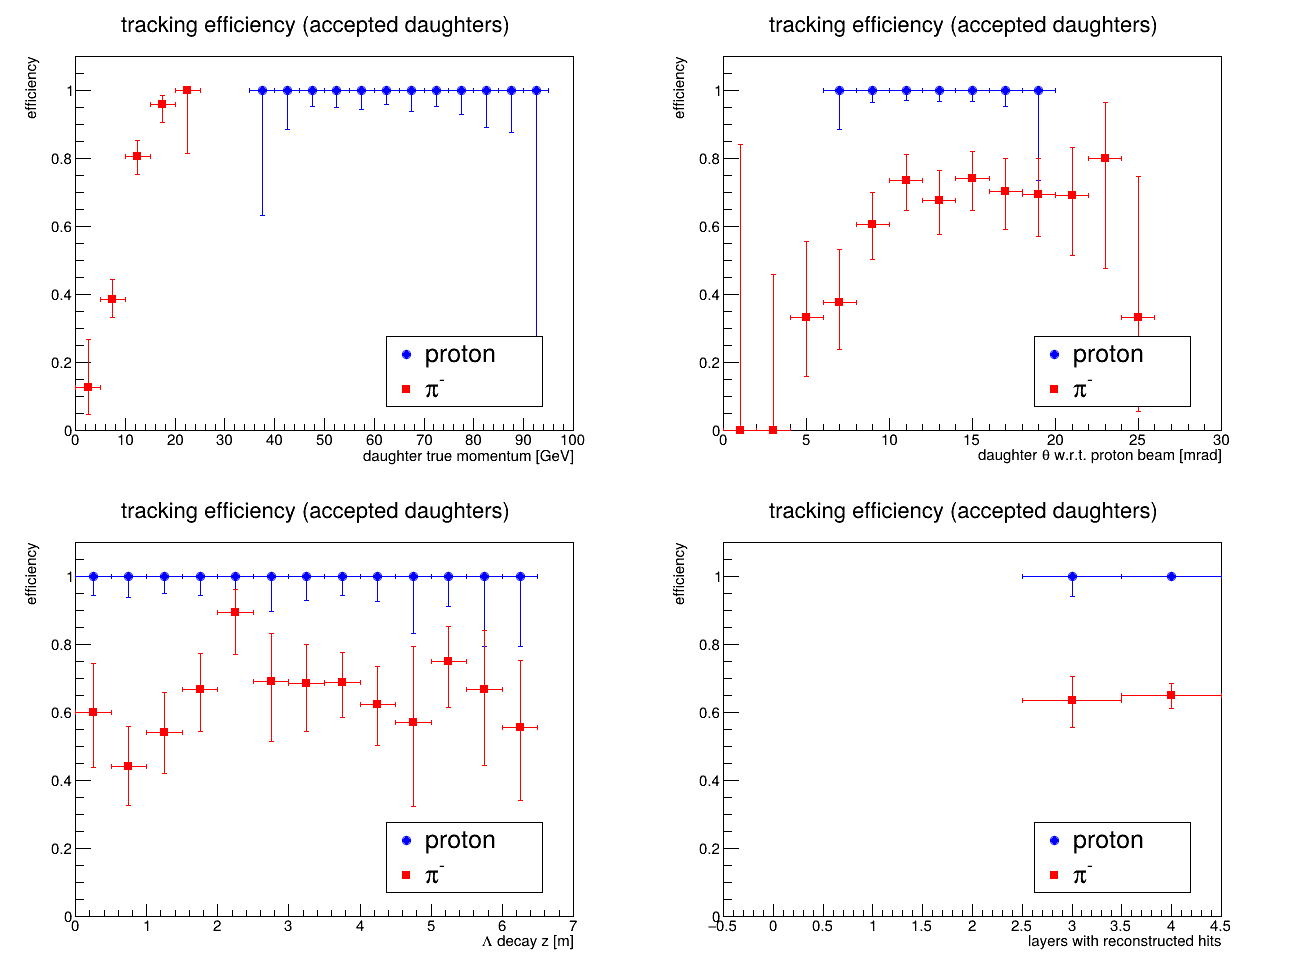
\includegraphics[width=\textwidth]{07_hit_seeding/tracking_efficiency_new_hit.png}\caption{new geometry, hit seeding}\end{subfigure}
\begin{subfigure}{0.49\textwidth}\centering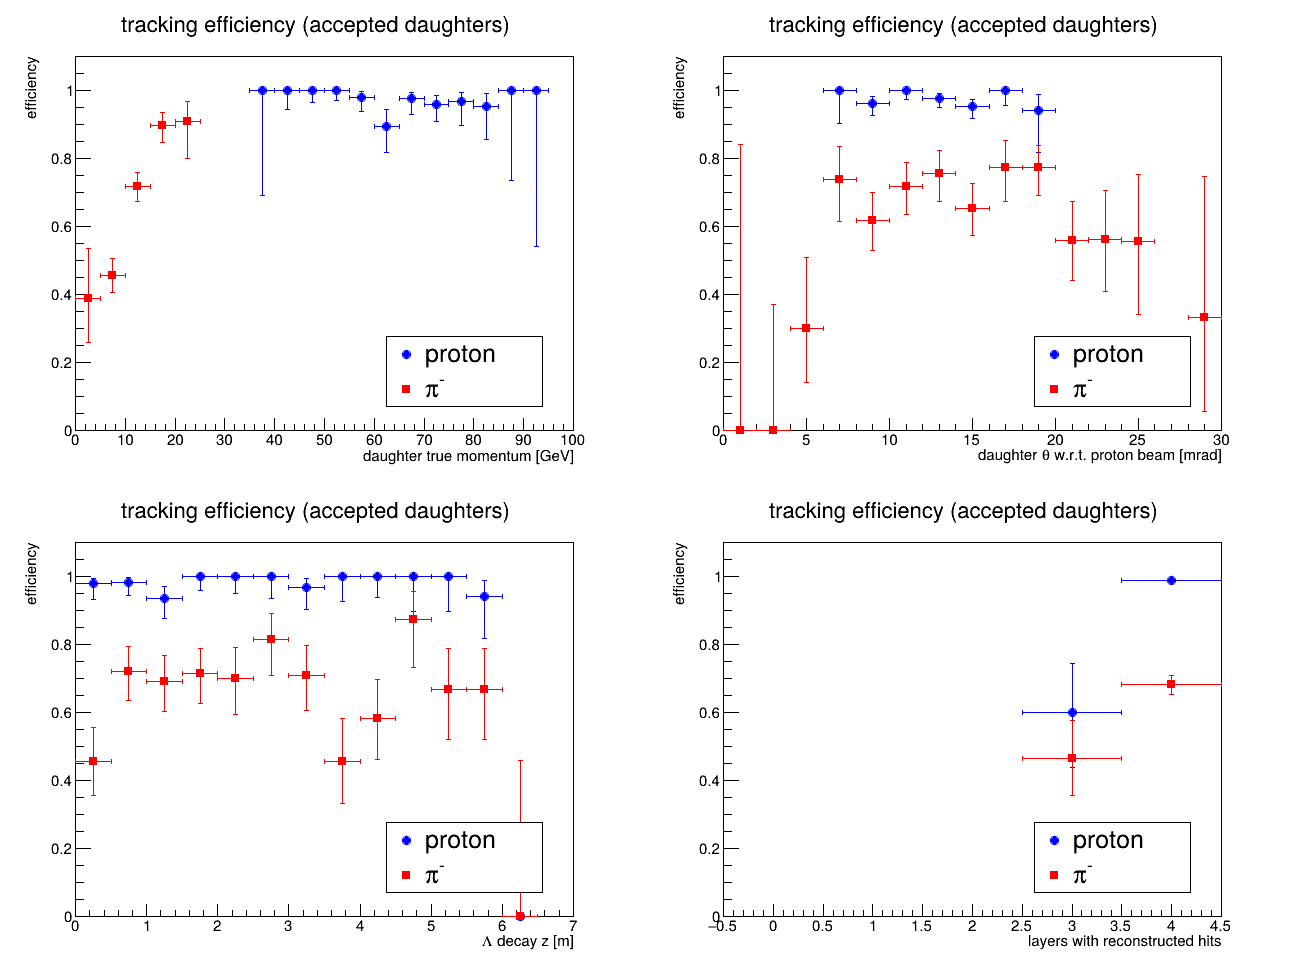
\includegraphics[width=\textwidth]{07_hit_seeding/tracking_efficiency_old_truth.png}\caption{old geometry, truth seeding}\end{subfigure}
\begin{subfigure}{0.49\textwidth}\centering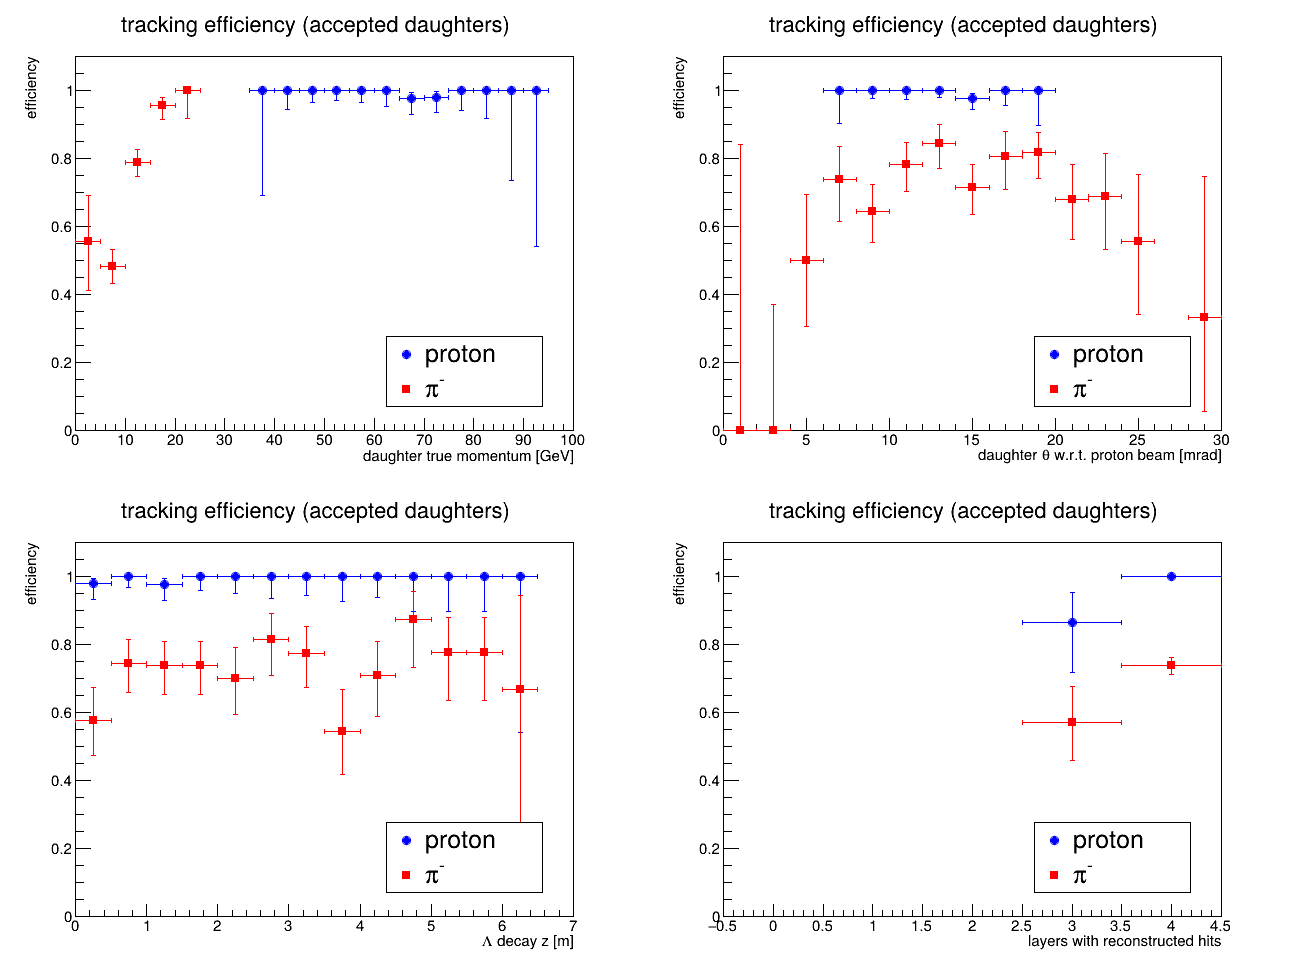
\includegraphics[width=\textwidth]{07_hit_seeding/tracking_efficiency_old_hit.png}\caption{old geometry, hit seeding}\end{subfigure}
\caption{Tracking efficiency of accepted daughters (proton blue, $\pi^-$ red) vs the daughter's
true momentum, its $\theta$, the $\Lambda$ decay $z$ and the number of layers with reconstructed hits.}
\label{fig:eff}
\end{figure}

\begin{itemize}
\item Hit seeding finds a seed for \emph{every} accepted daughter; with truth seeding 1--4\,\% have no
matching seed. With hit seeding every accepted proton is
reconstructed.
\item The $\pi^-$ is still lost in the CKF (seed $\to$ track), just as with truth seeding: of the
accepted $\pi^-$ of 5--10\,GeV only 39\,\% (new) and 48\,\% (old) are reconstructed with hit
seeding, 35\,\% and 46\,\% with truth seeding. Since every one of them now has a seed made of its
own hits, \textbf{the soft-$\pi^-$ loss is not a seeding problem}.
\end{itemize}

\subsection{Acceptance $\times$ efficiency}
\begin{table}[H]
\centering
\caption{Acceptance $\times$ efficiency, first report vs this update. The acceptance is unchanged (same simulation): 80 / 69 / 63\,\% (old), 61 / 49 / 41\,\% (new), proton / $\pi^-$ / both.}
\label{tab:axe}
\setlength{\tabcolsep}{4pt}
\resizebox{\textwidth}{!}{%
\begin{tabular}{@{}lccc@{}}
\toprule
& first report: main \code{8b44cae}, truth & \#3116 build, truth & \#3116 build, \textbf{hit}\\
\midrule
\multicolumn{4}{@{}l}{\emph{old geometry}}\\
tracking efficiency, p / $\pi^-$ & 82.2 / 55.6\,\% & \textbf{97.5 / 66.5\,\%} & 99.5 / 72.5\,\%\\
$A\times\varepsilon$ both, per $p\pi^-$ decay & 29.8\,\% & \textbf{41.7\,\%} & 45.5\,\%\\
both reconstructed, per generated $\Lambda$ & 15.0\,\% & 21.0\,\% & \textbf{22.9\,\%}\\
\midrule
\multicolumn{4}{@{}l}{\emph{new geometry} (first report: 5\,keV by option)}\\
tracking efficiency, p / $\pi^-$ & 92.9 / 60.8\,\% & 93.2 / 60.8\,\% & 100 / 64.6\,\%\\
$A\times\varepsilon$ both, per $p\pi^-$ decay & 24.7\,\% & 24.7\,\% & 27.0\,\%\\
both reconstructed, per generated $\Lambda$ & 12.0\,\% & 12.0\,\% & \textbf{13.1\,\%}\\
\bottomrule
\end{tabular}}
\end{table}

\paragraph{New geometry.} Truth seeding with the \#3116 build reproduces the first report exactly
(the 5\,keV default of \#3084 equals the 5\,keV option used then). Hit seeding adds 11 fully
reconstructed $\Lambda$s per 1000 (12.0 $\to$ 13.1\,\%).

\paragraph{Old geometry: not understood.} With the same simulated events, truth-seeded tracking in
the old geometry is much more efficient with the \#3116 build than with main \code{8b44cae}
(proton 82.2 $\to$ 97.5\,\%, both daughters per generated $\Lambda$ 15.0 $\to$ 21.0\,\%), while
the new geometry does not move. Three things differ between the two reconstructions: EICrecon
(\code{8b44cae} $\to$ \code{1ca147b}: 10 days of main, plus \#3116), the eic-shell image (ACTS
and other libraries, nightly of 2026-11-02 $\to$ 11-07), and the epic build of the old geometry
(the container's copy $\to$ a local build of the same commit). The threshold is not the cause (it
makes no difference in the 300\,$\mu$m geometry). This has not been investigated yet; until it is,
old-geometry numbers of the two reconstructions should not be compared with each other.

\begin{figure}[H]
\centering
\begin{subfigure}{0.49\textwidth}\centering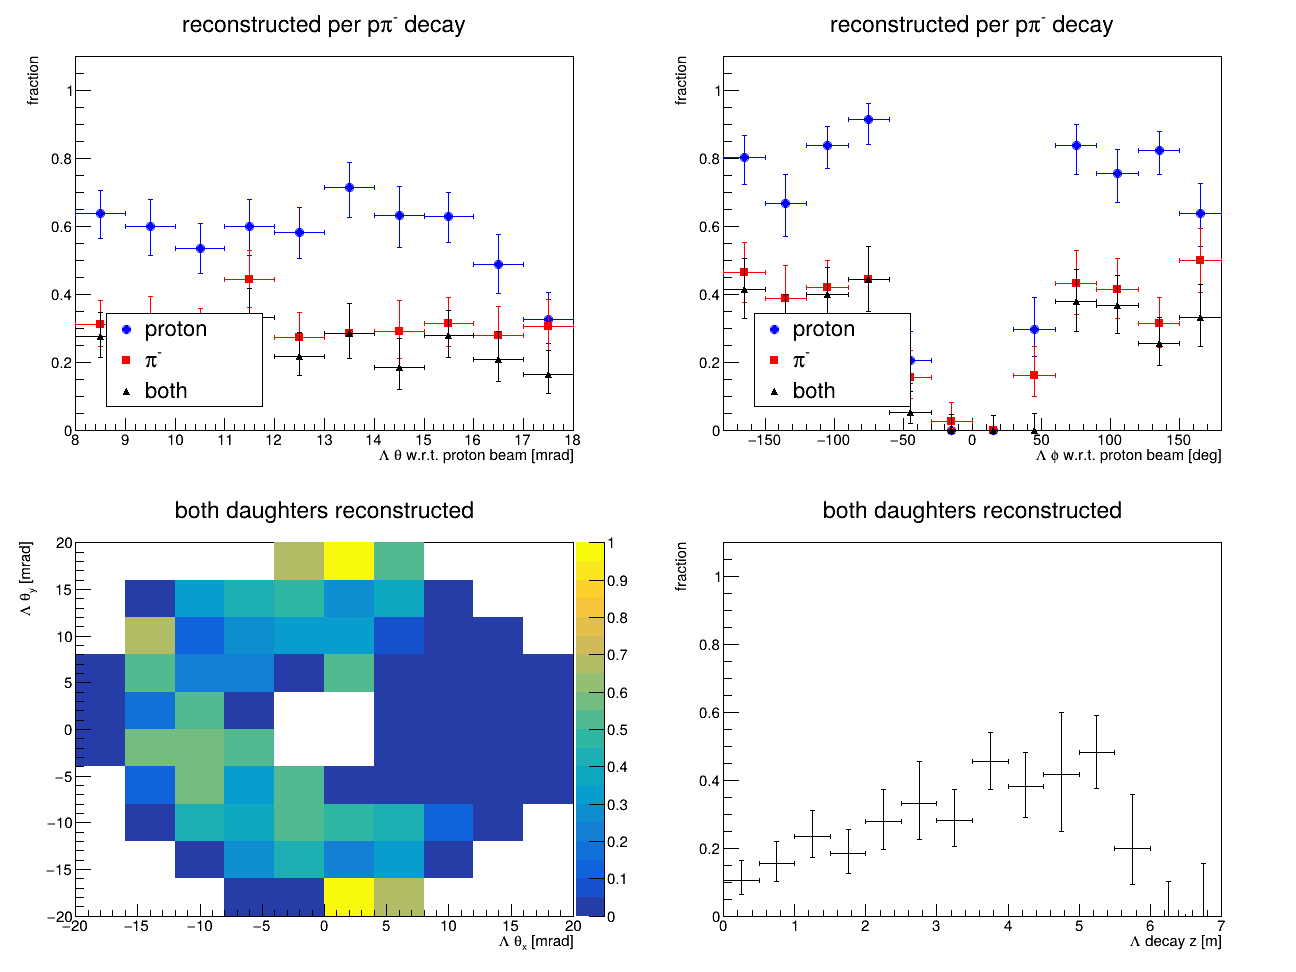
\includegraphics[width=\textwidth]{07_hit_seeding/acceptance_x_efficiency_new_truth.png}\caption{new geometry, truth seeding}\end{subfigure}
\begin{subfigure}{0.49\textwidth}\centering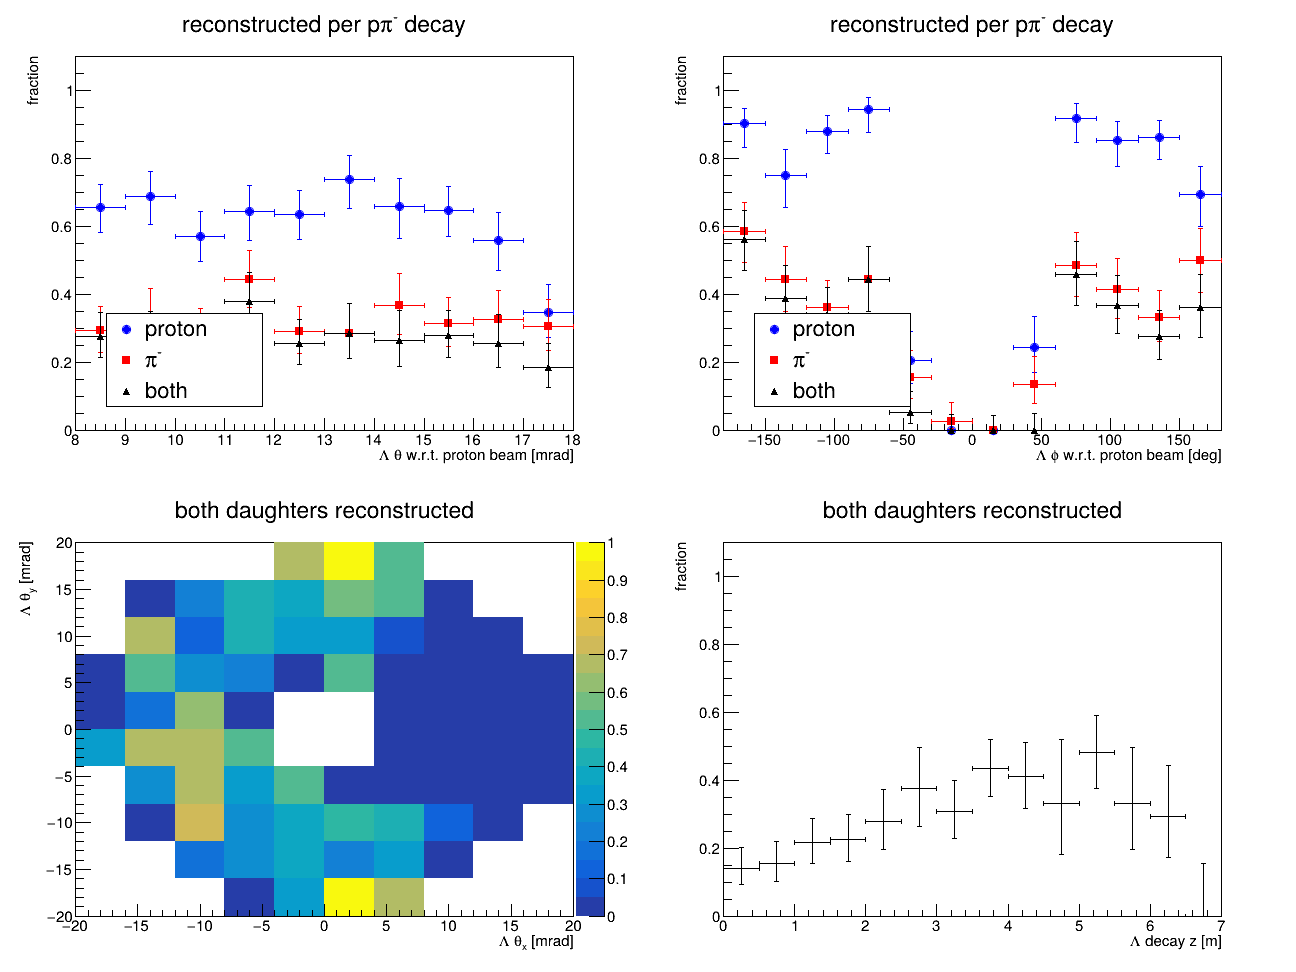
\includegraphics[width=\textwidth]{07_hit_seeding/acceptance_x_efficiency_new_hit.png}\caption{new geometry, hit seeding}\end{subfigure}
\caption{Acceptance $\times$ efficiency per $p\pi^-$ decay vs the $\Lambda$ $\theta$, $\phi$,
($\theta_x$, $\theta_y$) and decay $z$ (proton blue, $\pi^-$ red, both black).}
\end{figure}

%=====================================================================================
\section{The $\Lambda$ mass with hit-seeded tracks}

\begin{figure}[H]
\centering
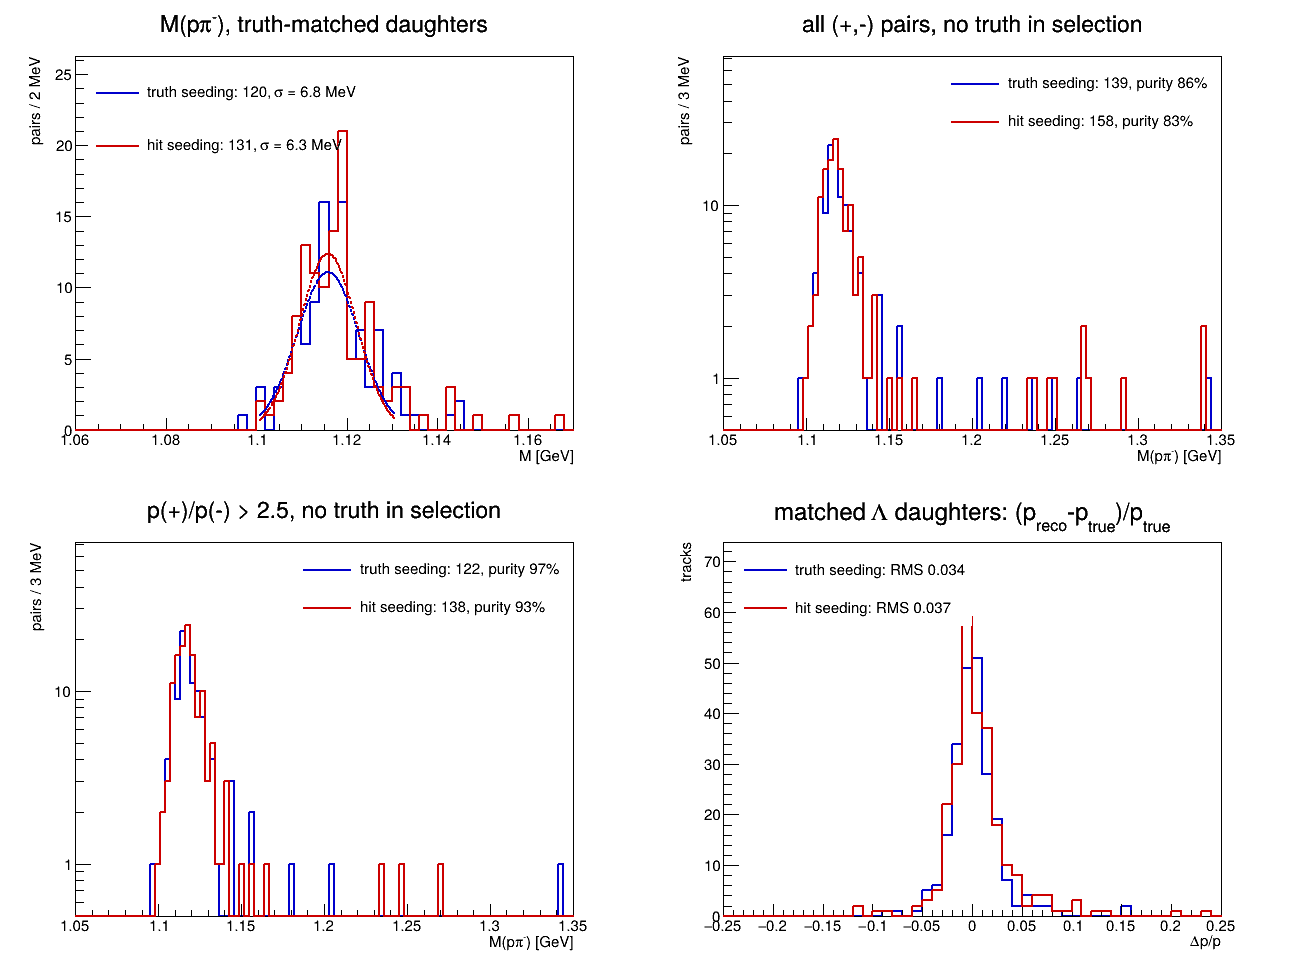
\includegraphics[width=0.75\textwidth]{07_hit_seeding/mass_seeding_compare_new.png}
\caption{New geometry: truth seeding (blue) vs hit seeding (red), same events
(\code{lambda_mass_seeding_compare.C}). Top: truth-matched $M(p\pi^-)$ with Gaussian fits; all
$(+,-)$ pairs (log scale). Bottom: pairs after $p(+)/p(-) > 2.5$; $\Delta p/p$ of the matched
daughters.}
\label{fig:masscmp}
\end{figure}

\begin{table}[H]
\centering
\caption{Mass and selection without truth, truth vs hit seeding (\#3116 build, 1000 $\Lambda$ per geometry).}
\setlength{\tabcolsep}{4pt}
\begin{tabular}{@{}lcccc@{}}
\toprule
& old, truth & old, hit & new, truth & new, hit\\
\midrule
truth-matched pairs & 210 & 229 & 120 & 131\\
Gaussian mean [GeV] & 1.1174 & 1.1175 & 1.1159 & 1.1159\\
Gaussian $\sigma$ [MeV] & 6.9 & 6.8 & 6.8 & 6.3\\
$\Delta p/p$ of the daughters, RMS & 3.8\,\% & 4.4\,\% & 3.4\,\% & 3.7\,\%\\
\midrule
reconstructed tracks (``other'' = not a $\Lambda$ daughter) & 824 (198) & 1097 (432) & 496 (68) & 548 (91)\\
all $(+,-)$ pairs / purity & 331 / 63\,\% & 877 / 26\,\% & 139 / 86\,\% & 158 / 83\,\%\\
after $p(+)/p(-) > 2.5$ / purity & 242 / 86\,\% & 348 / \textbf{64\,\%} & 122 / 97\,\% & 138 / \textbf{93\,\%}\\
$\pm 20$\,MeV window: signal / candidates & 200 / 207 & 206 / 219 & 110 / 110 & 116 / 116\\
\bottomrule
\end{tabular}
\end{table}

\begin{itemize}
\item \textbf{Same peak.} For the decays reconstructed with both seedings (old 209, new 114),
$M(\text{hit}) - M(\text{truth})$ has mean $\approx 0$ and RMS 4.4\,MeV. Hit seeding adds 17--20
decays and loses 1--6. The momentum resolution is slightly worse with hit seeding (3.7 vs 3.4\,\%
in the new geometry): the fitted tracks differ a little.
\item \textbf{More background.} Hit seeding also builds tracks for secondaries from interactions in
material; truth seeding only seeds charged MC particles produced inside its window (vertex
$z < 6$\,m, $|x|,|y| < 240$\,mm), presumably the reason for the difference (not checked). In the
old geometry, with 300\,$\mu$m sensors, this doubles the ``other'' tracks and the purity after the
momentum-ratio cut drops from 86 to 64\,\%; in the new geometry the effect is small (97 $\to$
93\,\%). The $\pm 20$\,MeV window stays $\ge 94$\,\% pure in all cases.
\item The +2\,MeV shift of the old geometry is still there with both seedings.
\end{itemize}

%=====================================================================================
\section{Sample composition: the right denominator}
\label{sec:fates}

The first report stated that 88--90\,\% of the $p\pi^-$ decays happen before the B0 tracker
($z < 5.8$\,m), and that the 24--25\,\% of $\Lambda$s with fate ``other'' interact in material
\emph{or leave the world volume}. The second part is wrong, and the first needs a comment. The
fates of the 1000 $\Lambda$s of the new-geometry sample (50--100\,GeV):

\begin{table}[H]
\centering
\begin{tabular}{@{}lccc@{}}
\toprule
fate & number & end at $z < 5.8$\,m & last end $z$\\
\midrule
decay to $p\pi^-$ & 485 & 438 & 8.7\,m\\
decay to $n\pi^0$ & 278 & 246 & 9.4\,m\\
other & 237 & 11 & 12.4\,m\\
\bottomrule
\end{tabular}
\end{table}

All 237 ``other'' $\Lambda$s have daughters, i.e.\ they \emph{interacted}; 205 of them end at
$z = 6$--10\,m. A $\Lambda$ that has not decayed by about 6\,m nearly always interacts in the
material downstream before it can decay. The $p\pi^-$ decays that exist are therefore mostly early
ones, and ``90\,\% before the B0'' is a fraction of the $p\pi^-$ decays, not of the $\Lambda$s.
Per generated $\Lambda$ the exponential decay law holds: 684 of 1000 (68\,\%) decay before
5.8\,m, against 66\,\% from $1 - e^{-L/\lambda}$ averaged over 50--100\,GeV, and 43.8\,\% decay
to $p\pi^-$ there, against $0.641 \times 66\,\% = 42\,\%$.

\textbf{Consequence:} results ``per $p\pi^-$ decay'' (acceptance, $A\times\varepsilon$) are
conditional on the decay having happened in the simulated region. ``Per generated $\Lambda$'' is
the unbiased figure and is used below.

%=====================================================================================
\section{$\Lambda$s up to 275\,GeV}

\subsection{Samples and expectation}
Two new samples per geometry, 500 events each (seeds 201, 202), with the same gun but
$p = 100$--275\,GeV (\code{PMIN=100 PMAX=275 lambda_sample.sh}, simulation only, then
\code{lambda_rereco.sh} with the \#3116 build). Together with the 50--100\,GeV samples they cover
50--275\,GeV; \code{lambda_vs_momentum.C} reads both.

The mean decay length is $\lambda = (p/m)\,c\tau = p[\text{GeV}] \times 7.07$\,cm
($c\tau = 7.89$\,cm, $m = 1.1157$\,GeV). The probability to decay before the B0 ($L = 5.8$\,m; the
path equals $z$ to $10^{-4}$ at $\sim 10$\,mrad) is $1 - e^{-L/\lambda}$: 81\,\% at 50\,GeV,
56\,\% at 100\,GeV, 34\,\% at 200\,GeV and 26\,\% at 275\,GeV. At beam-like momenta most $\Lambda$s
thus reach the B0 undecayed. On the other hand the $\pi^-$ carries 6--25\,\% of $p_\Lambda$, so at
high momentum it is no longer soft.

\subsection{Results}
\begin{figure}[H]
\centering
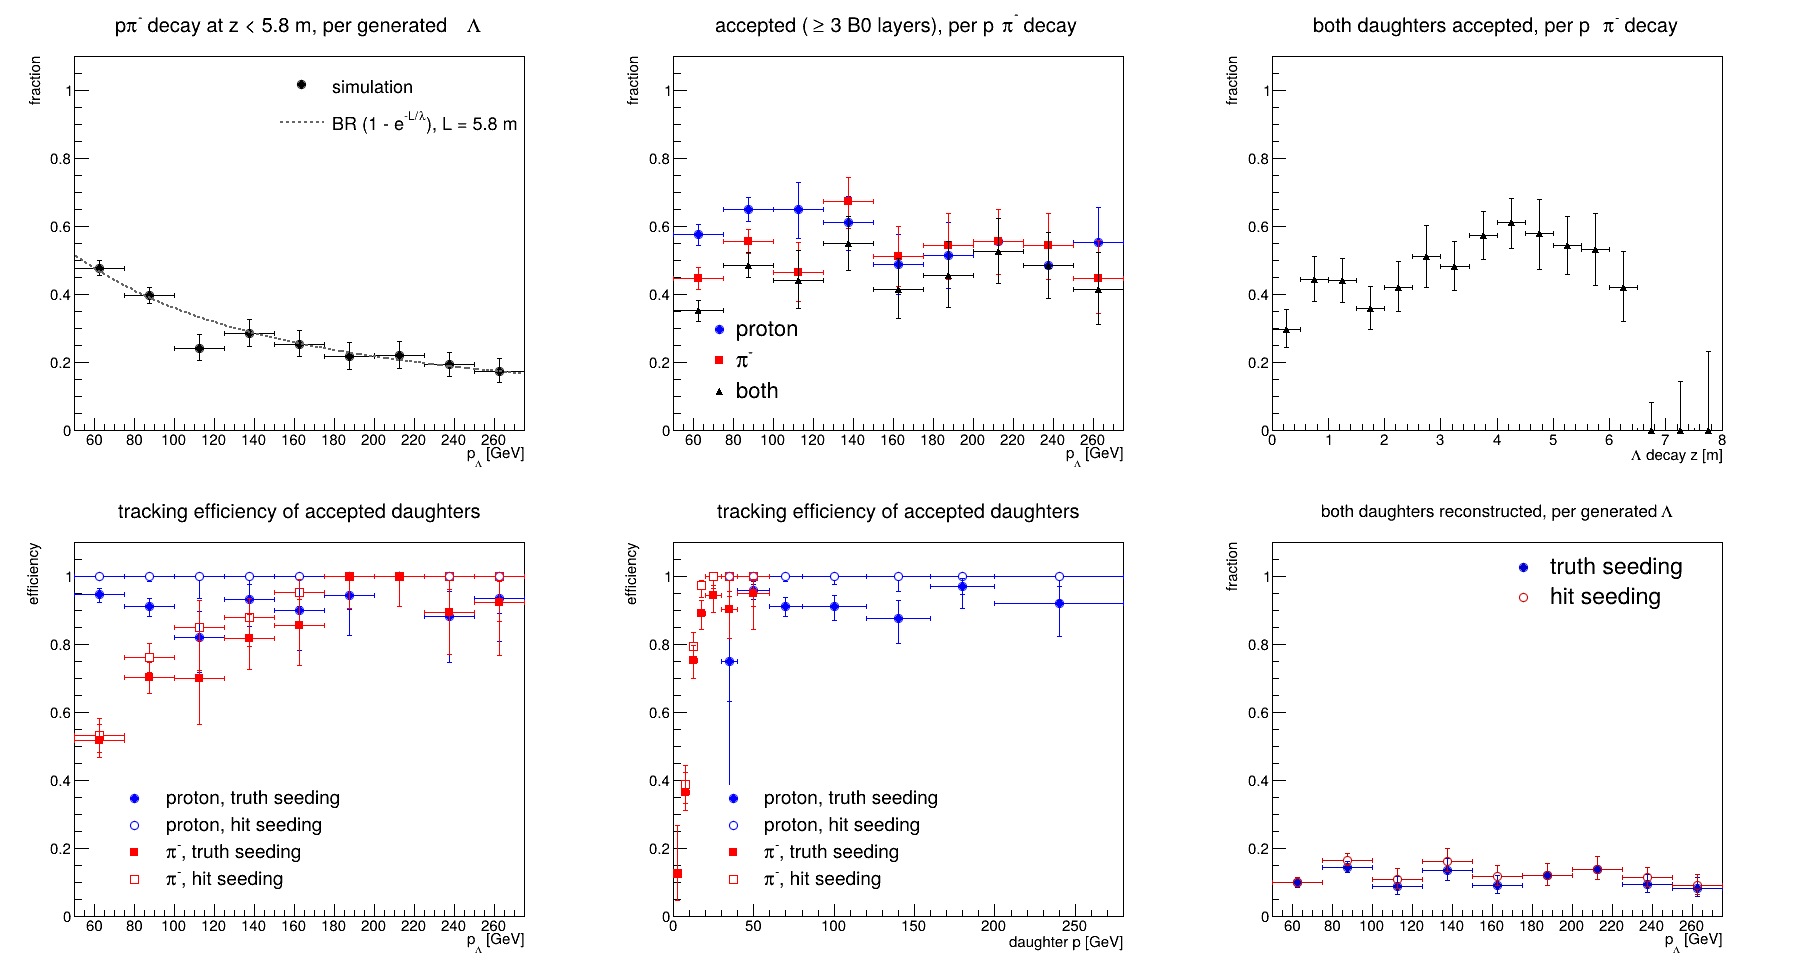
\includegraphics[width=\textwidth]{08_momentum/vs_momentum_new.png}
\caption{New geometry, 50--275\,GeV, \#3116 build. Top: $p\pi^-$ decays at $z < 5.8$\,m per
generated $\Lambda$ with the decay-law expectation (dashed); daughter acceptance per $p\pi^-$
decay vs $p_\Lambda$; acceptance of both daughters vs decay $z$. Bottom: tracking efficiency of
accepted daughters vs $p_\Lambda$ and vs the daughter's own momentum (filled: truth seeding, open:
hit seeding); both daughters reconstructed per generated $\Lambda$.}
\label{fig:pnew}
\end{figure}
\begin{figure}[H]
\centering
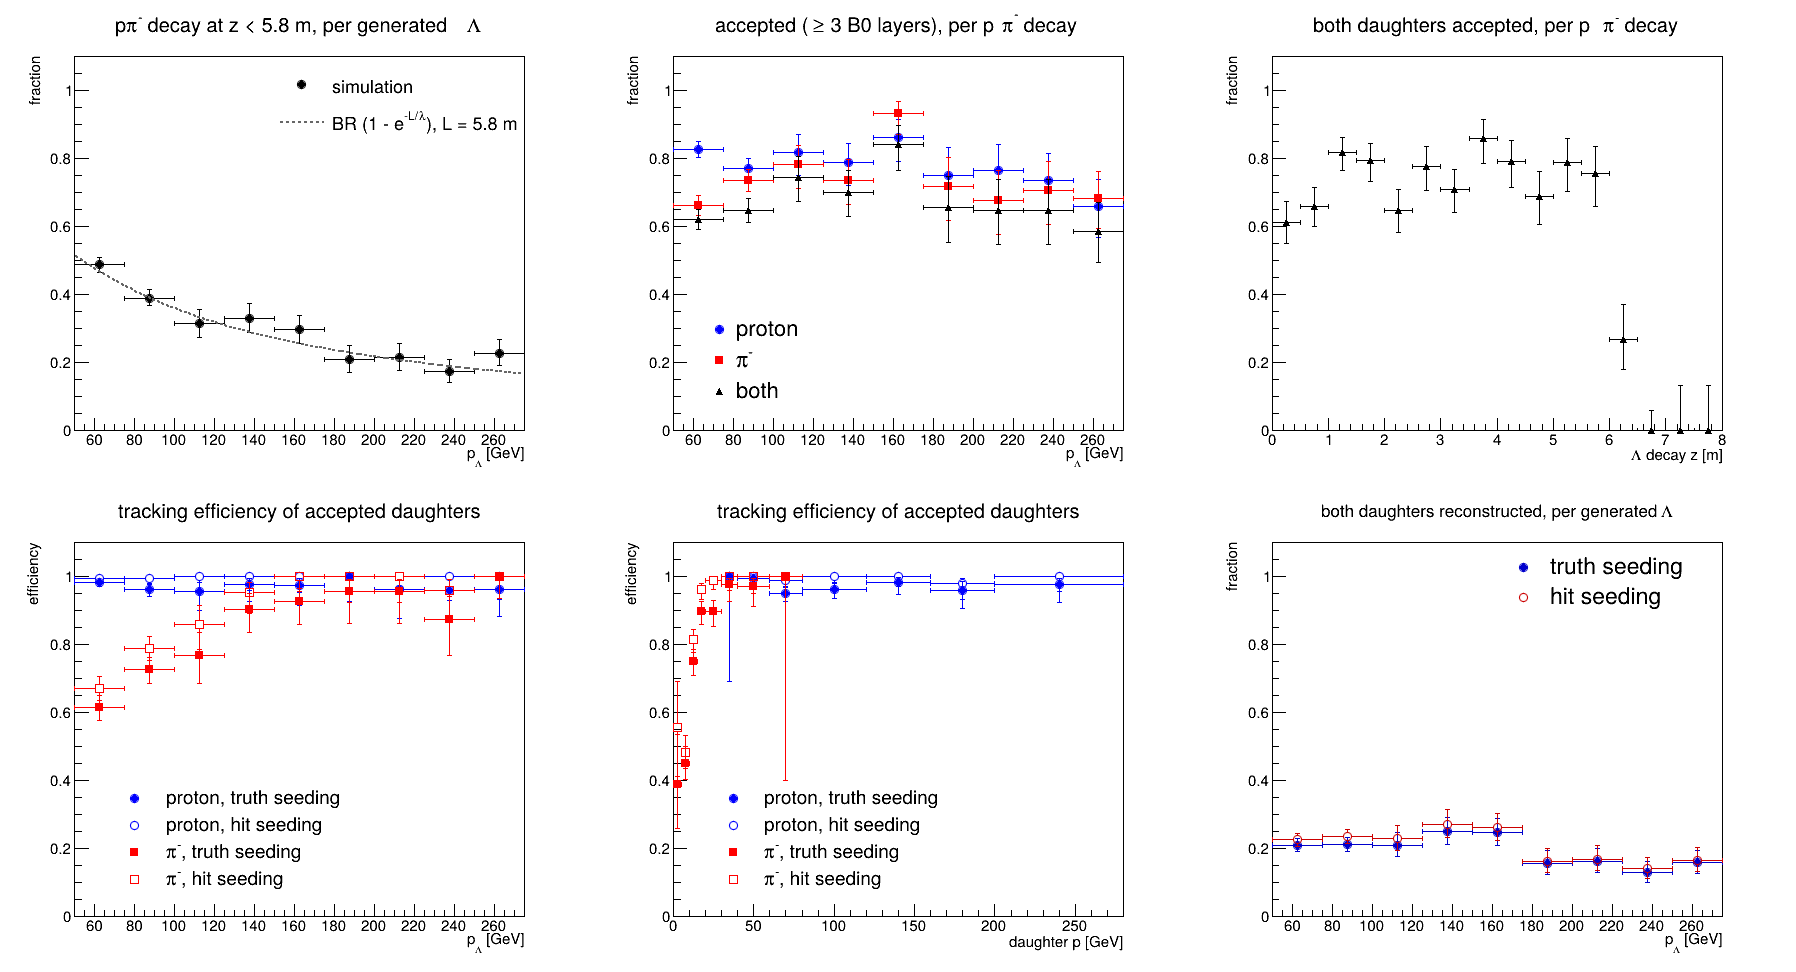
\includegraphics[width=\textwidth]{08_momentum/vs_momentum_old.png}
\caption{As Fig.~\ref{fig:pnew}, old geometry.}
\end{figure}

\begin{table}[H]
\centering
\caption{Per 25\,GeV bin of $p_\Lambda$ (about 500 $\Lambda$ per bin below 100\,GeV, 130--155 above): $p\pi^-$ decays at $z < 5.8$\,m per generated $\Lambda$ (simulated / decay law), both daughters accepted per $p\pi^-$ decay, tracking efficiency of accepted p and $\pi^-$ (truth / hit seeding), and both daughters reconstructed per generated $\Lambda$ (truth / hit).}
\label{tab:mom}
\setlength{\tabcolsep}{3.5pt}
\resizebox{\textwidth}{!}{%
\begin{tabular}{@{}l|cccccc|cccccc@{}}
\toprule
& \multicolumn{6}{c|}{old geometry} & \multicolumn{6}{c}{new geometry}\\
$p_\Lambda$ [GeV] & decay & law & acc.\ both & $\varepsilon_p$ & $\varepsilon_\pi$ & \textbf{both rec.} & decay & law & acc.\ both & $\varepsilon_p$ & $\varepsilon_\pi$ & \textbf{both rec.}\\
\midrule
50--75   & 49 & 47 & 62 & 98/100 & 62/67  & 21/23 & 48 & 47 & 35 & 95/100  & 52/53  & 10/10\\
75--100  & 39 & 39 & 65 & 96/99  & 73/79  & 21/23 & 40 & 39 & 49 & 91/100  & 70/76  & 14/17\\
100--125 & 31 & 33 & 75 & 96/100 & 77/86  & 21/23 & 24 & 33 & 44 & 82/100  & 70/85  & 9/11\\
125--150 & 33 & 29 & 70 & 98/100 & 91/95  & 25/27 & 28 & 29 & 55 & 93/100  & 82/88  & 14/16\\
150--175 & 30 & 25 & 84 & 97/100 & 93/100 & 25/26 & 25 & 25 & 42 & 90/100  & 86/95  & 9/12\\
175--200 & 21 & 23 & 66 & 100/100& 96/100 & 15/16 & 22 & 23 & 46 & 94/100  & 100/100& 12/12\\
200--225 & 21 & 21 & 65 & 96/96  & 96/100 & 16/17 & 22 & 21 & 53 & 100/100 & 100/100& 14/14\\
225--250 & 17 & 19 & 65 & 96/100 & 88/96  & 13/14 & 19 & 19 & 49 & 88/100  & 90/100 & 9/11\\
250--275 & 23 & 17 & 60 & 96/100 & 100/100& 16/17 & 18 & 17 & 43 & 94/100  & 93/100 & 9/10\\
\bottomrule
\end{tabular}}
\end{table}
All numbers in \%. Above 100\,GeV each bin has only 30--55 $p\pi^-$ decays, so the statistical
errors are 5--10 percentage points.

\begin{itemize}
\item \textbf{Decay before the B0} follows the decay law over the whole range, 48\,\% $\to$
17--18\,\% of the generated $\Lambda$s (as $p\pi^-$).
\item \textbf{Tracking efficiency rises.} The $\pi^-$ efficiency vs its own momentum goes from
$\approx 40$\,\% below 5\,GeV to $\approx 100$\,\% above $\approx 20$\,GeV for both seedings; vs
$p_\Lambda$ it rises from 52--67\,\% at 50--75\,GeV to 90--100\,\% above 150\,GeV. Protons: 100\,\%
with hit seeding at all momenta; truth seeding loses 5--10\,\% in the new geometry.
\item \textbf{Acceptance} of both daughters per $p\pi^-$ decay stays at 60--85\,\% (old) and
35--55\,\% (new); in the new geometry it is limited by the sensor coverage ($\phi$ gap), not by
the momentum. Decays beyond $z \approx 6.5$\,m are never accepted (fewer than three layers left).
\item \textbf{Net effect: roughly flat.} Both daughters reconstructed per generated $\Lambda$:
old 21--27\,\% up to 175\,GeV and 13--17\,\% above; new 9--17\,\% over the whole range. The
falling decay probability is compensated by the better reconstruction of the early decays: in the
new geometry 21\,\% of the early $p\pi^-$ decays are fully reconstructed at 50--75\,GeV, about
40--60\,\% above 150\,GeV.
\end{itemize}

\subsection{Differences between the 50--100 and 100--275\,GeV samples}
Same gun (apart from the momentum), same geometries at the same commits and the same
reconstruction (\#3116 build) for both. The simulation, however, ran in different eic-shell images
(2026-11-02 and 11-07), and the old geometry came from the container in the first case and from a
local build of the same commit in the second; given the unexplained old-geometry difference above,
the old-geometry curves across 100\,GeV carry that caveat. The new-geometry results were stable
under the same changes. The 100--275\,GeV files are about three times larger per event
(1.2--1.5\,GB per 500 events), presumably from the larger showers of energetic $\Lambda$s
interacting downstream (not checked).

%=====================================================================================
\section{Summary and open points}

\begin{itemize}
\item \textbf{Hit seeding (EICrecon\#3116) works for displaced $\Lambda$ daughters:} a seed for
every accepted daughter, every accepted proton reconstructed, 1--2 percentage points more fully
reconstructed $\Lambda$s than truth seeding (new geometry 12.0 $\to$ 13.1\,\% of the generated
$\Lambda$s), and the same mass peak ($\sigma \approx 6$--7\,MeV). It also tracks secondaries;
without truth the purity after the momentum-ratio cut is 93\,\% (new) and 64\,\% (old geometry).
\item \textbf{The soft-$\pi^-$ loss is in the CKF, not in the seeding}: it persists with a seed for
every $\pi^-$.
\item \textbf{5\,keV} is now the default B0 threshold (\#3084).
\item \textbf{Energetic $\Lambda$s:} fewer decay before the B0 (decay law), but those that do are
reconstructed better; the fully reconstructed fraction is roughly flat up to 275\,GeV.
\item \textbf{Denominator:} ``per generated $\Lambda$'' is the unbiased figure; ``per $p\pi^-$ decay''
is conditional on an early decay.
\end{itemize}

Open points: the jump of the old-geometry truth-seeded efficiency between EICrecon builds
(rerun \code{8b44cae} in the new image, or \code{1ca147b} with the container's old epic); the CKF
loss of soft tracks; the +2\,MeV mass shift in the old geometry; following \#3116 until it is
merged; events with other particles and beam background, where the decay vertex will be needed.

%=====================================================================================
\appendix
\section{Reproducing}
\begin{itemize}
\item Builds: \code{scripts/build/build_eicrecon.sh EICrecon_pr3116 3116} (a PR) and
\code{scripts/build/build_epic.sh epic_43f427e <full commit>} (a commit). \code{GEO} and \code{RECO}
of the scripts accept a directory name under \code{\$EIC_TOP} or \code{/opt/detector}.
\item Re-reconstruction: \code{scripts/production/lambda_rereco.sh <GEO> <NAME> EICrecon_pr3116 eicreconpr3116 [EXTRA] [DEST]}.
\item High-momentum samples: \code{PMIN=100 PMAX=275 SIM_ONLY=1 scripts/production/lambda_sample.sh ...}.
\item Results: \code{scripts/make_results.sh 07 08}. Files on EOS: \code{lambda_1000ev/*.eicreconpr3116.*},
\code{lambda_100to275/}.
\item Pitfall: JANA keeps the \emph{first} value of a repeated \code{-P} option, so
\code{-Pjana:nevents=20} after \code{-Pjana:nevents=-1} is ignored.
\end{itemize}

\end{document}
